\chapter{LAB Session 04 -- Low Voltage Band-Gap Voltage Reference}

\section{Preliminary Design of the LV-BGR}

\subsection{LV-BGR Schematic}

\begin{figure}[H]
    \centering
    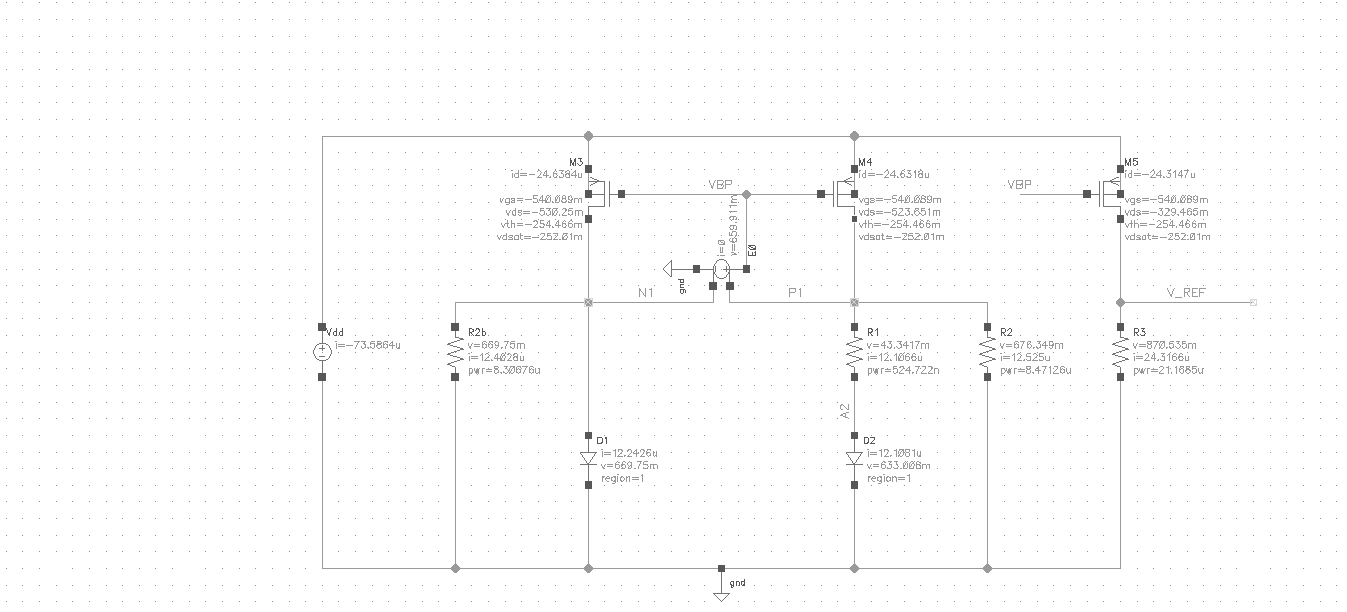
\includegraphics[width=\linewidth]{chapters/lab04/Schematic_LV_BGR.png}
    \caption{Schematic of the implemented LV-BGR.}
    \label{fig:lv_bgr_schematic}
\end{figure}

\subsection{Initial Sizing}

The preliminary design was obtained by imposing $I_1=10\,\mu\mathrm{A}$ and $N=\frac{A_{D2}}{A_{D1}}=4$. Since the OTA equalizes the two upper node voltages, the voltage across $R_1$ is $V_{R1}=V_{D1}-V_{D2}=U_T\ln(N)$, yielding $R_1=\frac{U_T\ln(N)}{I_1}\approx3.58\,\mathrm{k}\Omega$. Using the diode equation, the forward voltage of $D_1$ is estimated as $V_{D1}\approx0.665\,\mathrm{V}$.

The resistor $R_2$ controls the PTAT compensation term. Imposing $\frac{\partial V_{REF}}{\partial T}\approx0$ gives $R_2 = R_1 \frac{\ln(I_{S0}/I_1)}{\ln(N)} \approx54\,\mathrm{k}\Omega$. Finally, $R_3$ scales the output voltage to $V_{REF}=0.8\,\mathrm{V}$, requiring $R_3\approx35.8\,\mathrm{k}\Omega$. All resistors were implemented with a temperature coefficient of $TC_R=-5\cdot10^{-4}\,\mathrm{K}^{-1}$.

\subsection{PMOS Current Mirror Sizing}

The PMOS devices $M_3$, $M_4$, and $M_5$ form the bias current mirror. To reduce channel-length modulation, all transistors were initialized with $L=1.2\,\mu\mathrm{m}$. 

The mirror current is approximately $I_D=I_1+I_2$, where $I_2=\frac{V_{D1}}{R_2}\approx12.3\,\mu\mathrm{A}$, yielding $I_D\approx22.3\,\mu\mathrm{A}$. Assuming $|V_{OV}|=0.25\,\mathrm{V}$ for all transistors, the PMOS widths are estimated from the saturation current equation:
\[
W=\frac{2LI_D}{k_pV_{OV}^2}\approx8.6\,\mu\mathrm{m}
\]

\begin{table}[H]
\centering
\begin{tabular}{|c|c|c|c|}
\hline
\textbf{Component} & \textbf{R [k$\Omega$]} & \textbf{L [$\mu$m]} & \textbf{W [$\mu$m]} \\
\hline
M3 & -- & 1.2 & 8.6 \\
M4 & -- & 1.2 & 8.6 \\
M5 & -- & 1.2 & 8.6 \\
R1 & 3.58 & -- & -- \\
R2 & 54 & -- & -- \\
R3 & 35.8 & -- & -- \\
\hline
\end{tabular}
\caption{Initial sizing parameters of the LV-BGR.}
\label{tab:lvbgr_initial_sizing}
\end{table}

\subsection{PTAT and CTAT Characterization}

All the following temperature coefficients were evaluated locally around $27^\circ\mathrm{C}$, using close markers, since some curves are not perfectly linear. A DC temperature sweep from $-40^\circ\mathrm{C}$ to $85^\circ\mathrm{C}$ was performed to verify the CTAT and PTAT quantities.

\begin{figure}[H]
    \centering
    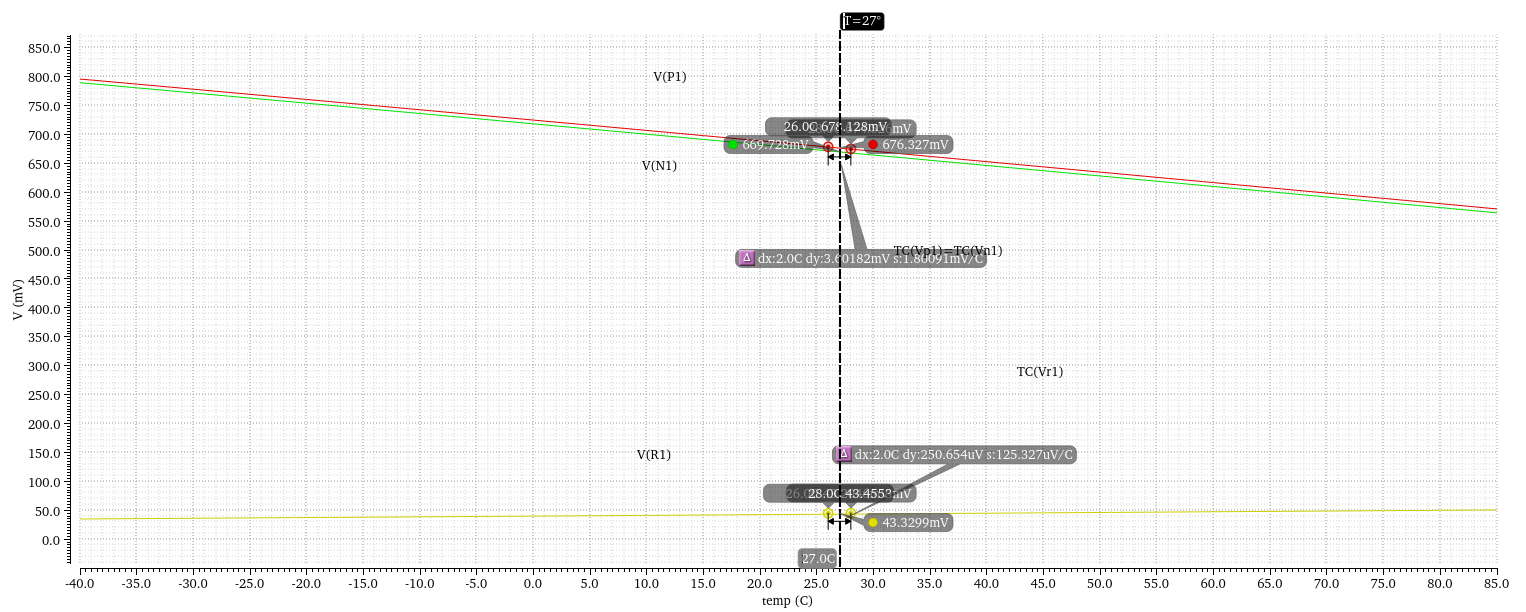
\includegraphics[width=\linewidth]{chapters/lab04/plot1.png}
    \caption{CTAT node voltages and PTAT voltage across $R_1$.}
    \label{fig:plot1}
\end{figure}

The diode voltages $V_{N1}$ and $V_{P1}$ show the expected CTAT behavior:
\[
\frac{dV_D}{dT}\approx -1.80\,\mathrm{mV/^\circ C}.
\]
The voltage across $R_1$, $V_{PTAT}=V(P1)-V(A2)$, increases with temperature, confirming the PTAT generation:
\[
\frac{dV_{PTAT}}{dT}\approx 125\,\mu\mathrm{V/^\circ C}.
\]

\subsection{Current Characterization}

\begin{figure}[H]
    \centering
    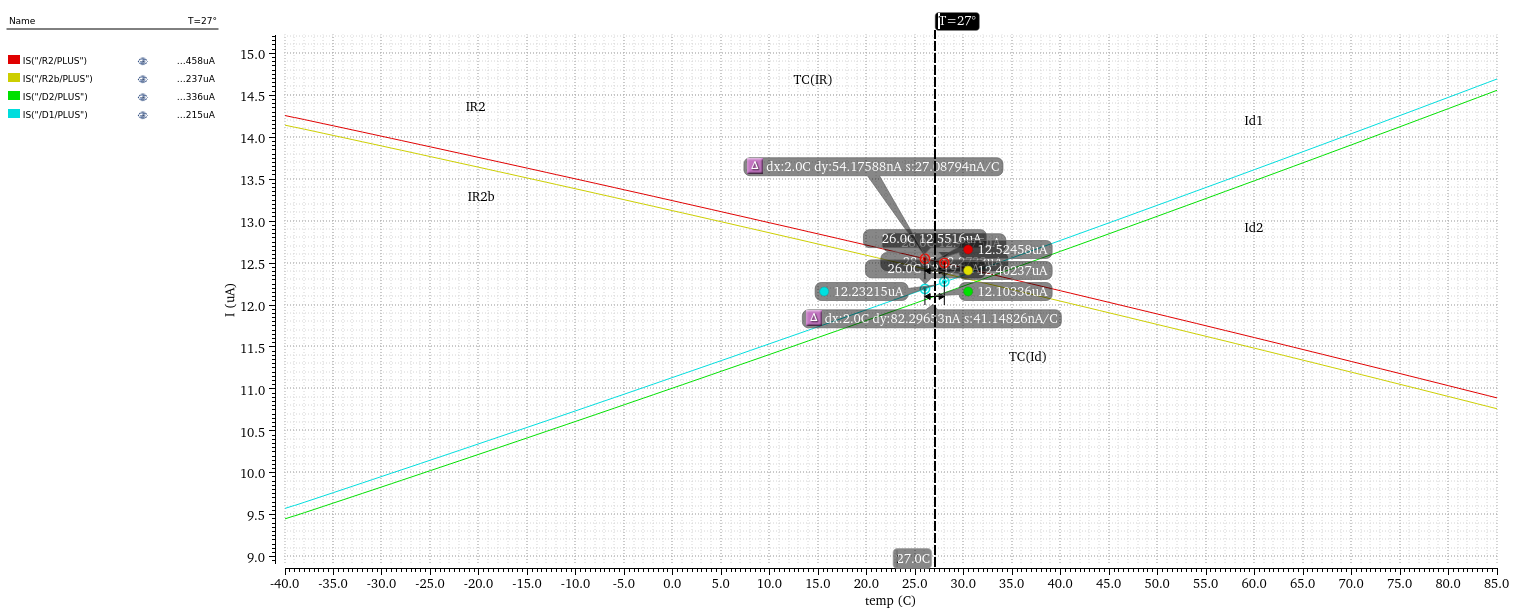
\includegraphics[width=\linewidth]{chapters/lab04/plot2.png}
    \caption{Internal branch currents versus temperature.}
    \label{fig:plot2}
\end{figure}

The diode currents $I_{D1}$ and $I_{D2}$ are almost equal, confirming the correct operation of the OTA feedback loop and of the PMOS current mirror. Around room temperature, the extracted slopes are approximately:
\[
\frac{dI_D}{dT}\approx 41\,\mathrm{nA/^\circ C},
\qquad
\frac{dI_{R2}}{dT}\approx 27\,\mathrm{nA/^\circ C}.
\]
However, the simulated diode current is still larger than the target value $I_1=10\,\mu\mathrm{A}$, therefore $R_1$ must be tuned.

\subsection{Initial Reference Voltage Characterization}

\begin{figure}[H]
    \centering
    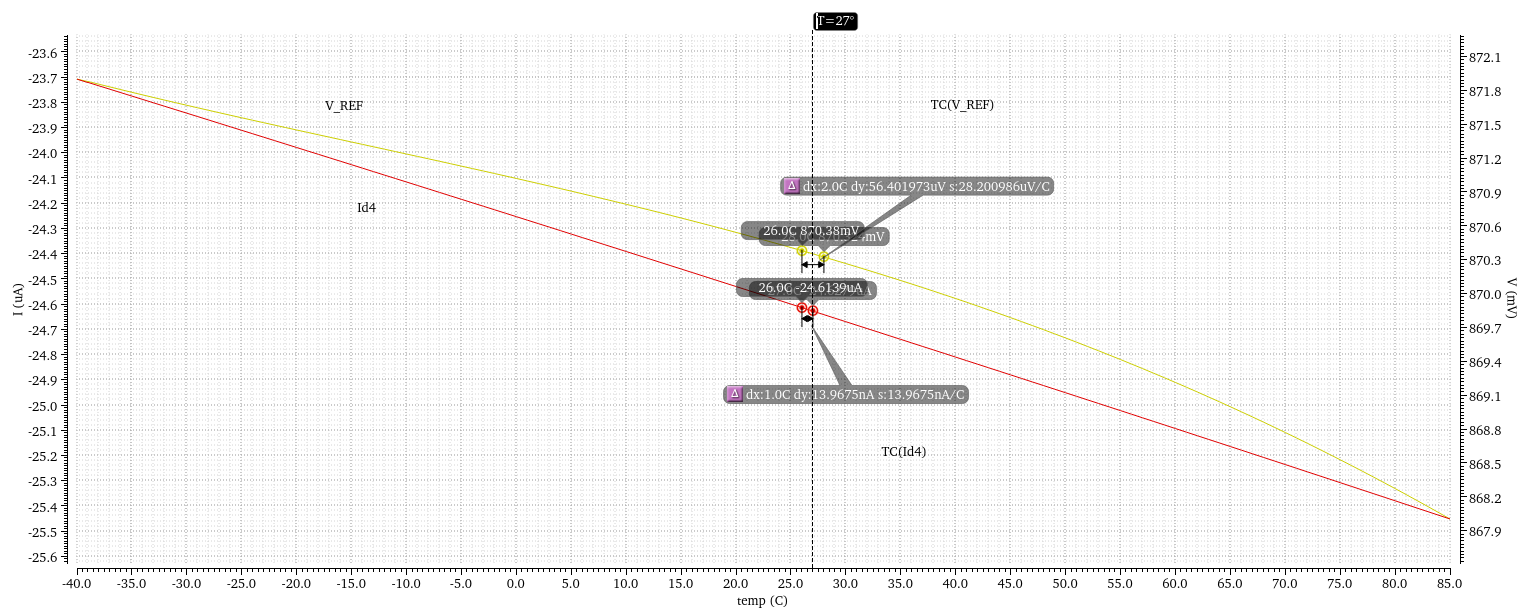
\includegraphics[width=\linewidth]{chapters/lab04/plot3.png}
    \caption{Initial $V_{REF}$ and $I_{D4}$ versus temperature.}
    \label{fig:plot3}
\end{figure}

The preliminary design generates a reference voltage close to the desired range, but still affected by a residual temperature dependence. Around $27^\circ\mathrm{C}$:
\[
V_{REF}\approx 870.4\,\mathrm{mV},
\]
\[
\frac{dV_{REF}}{dT}\approx 28.2\,\mu\mathrm{V/^\circ C},
\qquad
TC_{VREF}\approx 32\,\mathrm{ppm/^\circ C}.
\]
The PMOS mirror current shows a local slope of about:
\[
\frac{dI_{D4}}{dT}\approx 14\,\mathrm{nA/^\circ C}.
\]

\paragraph{Assessment of the Preliminary Design}
The preliminary design already exhibits the expected CTAT and PTAT behaviors. At room temperature, the simulated branch current is $I_{D1}=12.31\,\mu\mathrm{A}$, compared to the target value of $10\,\mu\mathrm{A}$, while the reference voltage is $V_{REF}=870.4\,\mathrm{mV}$ instead of the specified $800\,\mathrm{mV}$. Moreover, the extracted temperature coefficient is $TC_{VREF}\approx32\,\mathrm{ppm/^\circ C}$, which is significantly larger than the target specification. These deviations are mainly due to the approximations adopted in the hand calculations and to device non-idealities included in the simulation models. Therefore, a tuning procedure is required to meet the design specifications.


\section{Resistors Tuning}

The resistor values were then tuned sequentially. $R_1$ sets the PTAT current, $R_2$ controls the PTAT/CTAT compensation, and $R_3$ sets the final absolute value of $V_{REF}$.

\subsection{Tuning of $R_1$}

The theoretical value $R_1=3.58\,\mathrm{k}\Omega$ produced $I_{D1}=12.31\,\mu\mathrm{A}$, larger than the target current $I_1=10\,\mu\mathrm{A}$. Since the branch current is approximately inversely proportional to $R_1$, the resistor was increased to:
\[
\boxed{R_1=4.346\,\mathrm{k}\Omega}
\]
obtaining $I_{D1}=10.0018\,\mu\mathrm{A}$.

\begin{figure}[H]
    \centering
    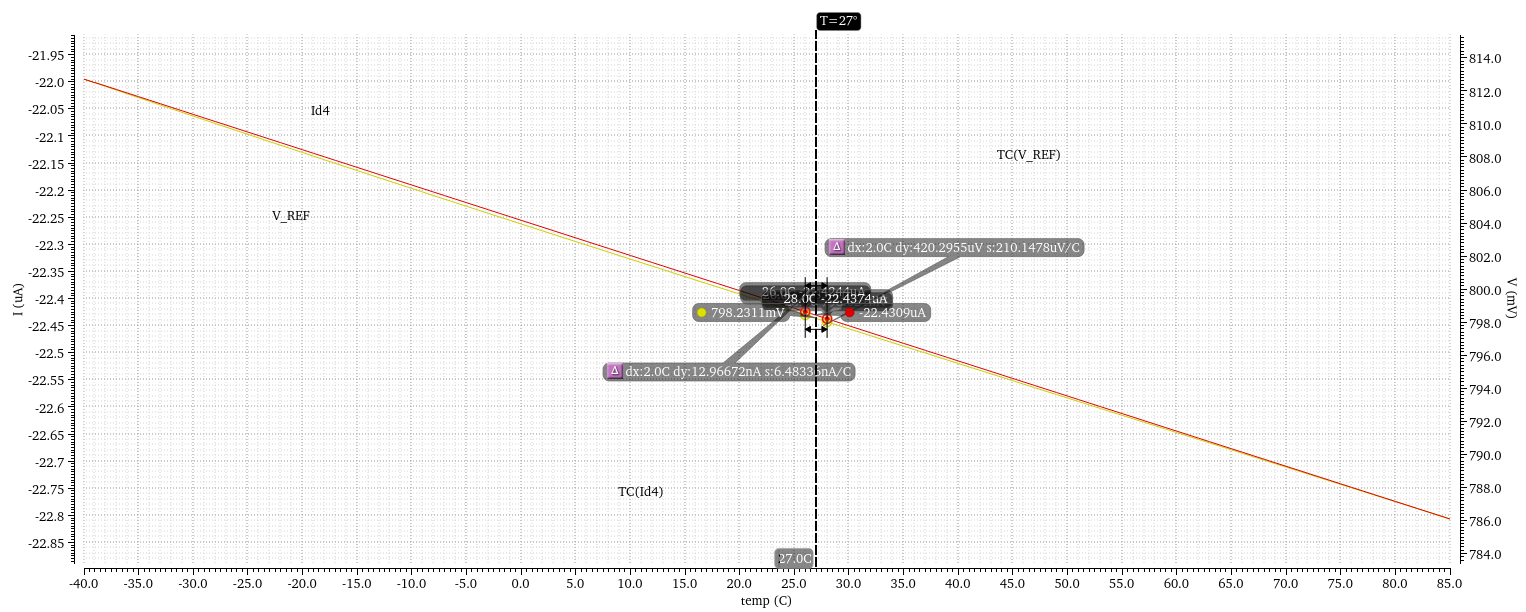
\includegraphics[width=\linewidth]{chapters/lab04/tuning1.png}
    \caption{$V_{REF}$ and $I_{D4}$ after tuning $R_1$.}
    \label{fig:tuning1}
\end{figure}

After this step, $V_{REF}$ still shows a significant temperature slope:
\[
\frac{dV_{REF}}{dT}\approx 210\,\mu\mathrm{V/^\circ C}.
\]
This indicates that the PTAT/CTAT compensation must be adjusted through $R_2$.

\subsection{Tuning of $R_2$}

The resistor $R_2$ controls the weight of the PTAT term added to the CTAT diode voltage:
\[
V_{REF}\propto V_{D1}+\frac{R_2}{R_1}U_T\ln(N).
\]
Therefore, increasing $R_2$ increases the PTAT contribution. A parametric sweep was performed on both matched resistors $R_2=R_{2b}$. First, a coarse sweep was performed:
\[
54\,\mathrm{k}\Omega \leq R_2 \leq 70\,\mathrm{k}\Omega,
\qquad
\Delta R_2=1\,\mathrm{k}\Omega.
\]

\begin{figure}[H]
    \centering
    \includegraphics[width=\linewidth]{chapters/lab04/tuning2a.png}
    \caption{Coarse parametric sweep of $R_2$.}
    \label{fig:tuning2a}
\end{figure}

The minimum local slope was found around $R_2=66\,\mathrm{k}\Omega$. A refined sweep was then performed around this region:
\[
64\,\mathrm{k}\Omega \leq R_2 \leq 70\,\mathrm{k}\Omega,
\qquad
\Delta R_2=0.2\,\mathrm{k}\Omega.
\]

\begin{figure}[H]
    \centering
    \includegraphics[width=\linewidth]{chapters/lab04/tuning2b.png}
    \caption{Refined parametric sweep of $R_2$.}
    \label{fig:tuning2b}
\end{figure}

The selected value is:
\[
\boxed{R_2=R_{2b}=66\,\mathrm{k}\Omega}.
\]

\begin{figure}[H]
    \centering
    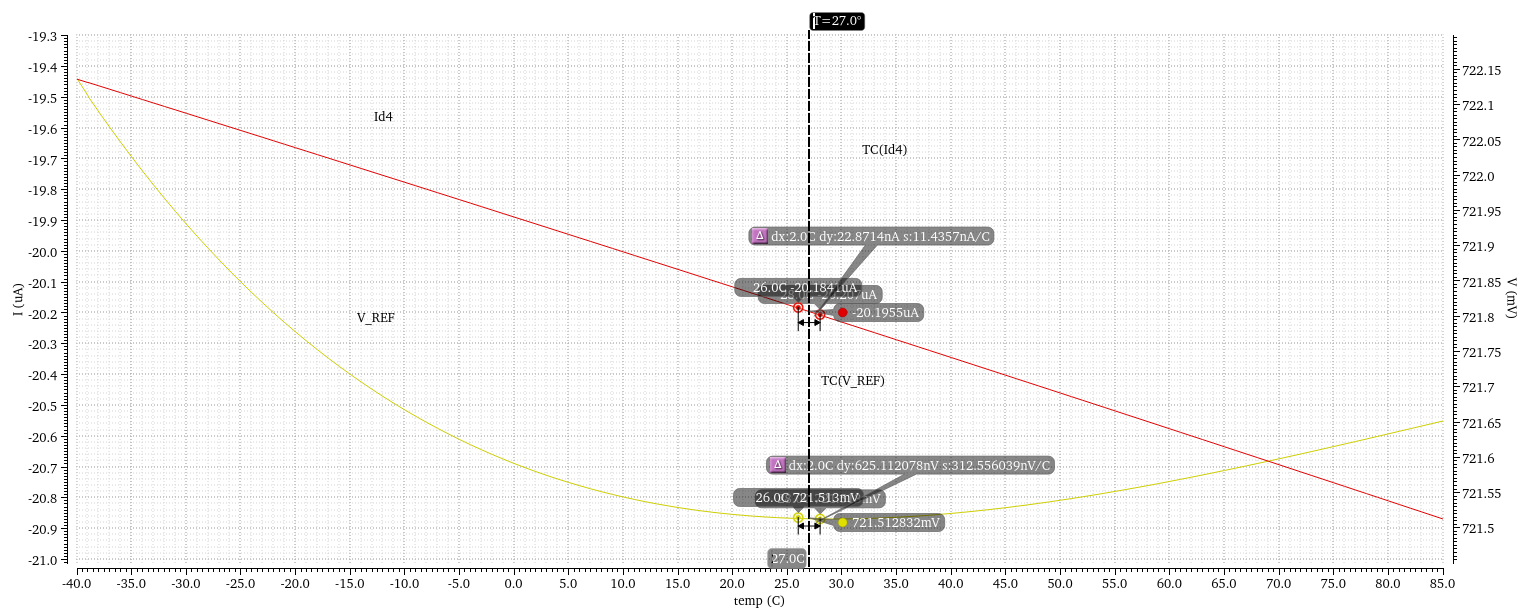
\includegraphics[width=\linewidth]{chapters/lab04/tuning2c.png}
    \caption{$V_{REF}$ and $I_{D4}$ after tuning $R_2$.}
    \label{fig:tuning2c}
\end{figure}

With this value, the local temperature coefficient of $V_{REF}$ is strongly reduced:
\[
\frac{dV_{REF}}{dT}\approx 0.31\,\mu\mathrm{V/^\circ C}.
\]
The resulting $V_{REF}(T)$ characteristic is not perfectly linear and exhibits a slight second-order curvature. This behavior is mainly due to second-order effects neglected in the hand calculations, especially the temperature dependence of model parameters such as $I_{S0}$. Nevertheless, the tuning of $R_2$ allows the operating point around room temperature to lie close to the minimum of the parabola, where the local temperature coefficient is minimized.

\subsection{Tuning of $R_3$}

After the compensation was optimized through $R_2$, $R_3$ was tuned to set the absolute value of the reference voltage. Since $V_{REF}\approx \frac{R_3}{R_2}V_{G0}$, $R_3$ directly scales the output reference. A parametric sweep was performed around the expected value:
\[
39.7\,\mathrm{k}\Omega \leq R_3 \leq 40.0\,\mathrm{k}\Omega.
\]

\begin{figure}[H]
    \centering
    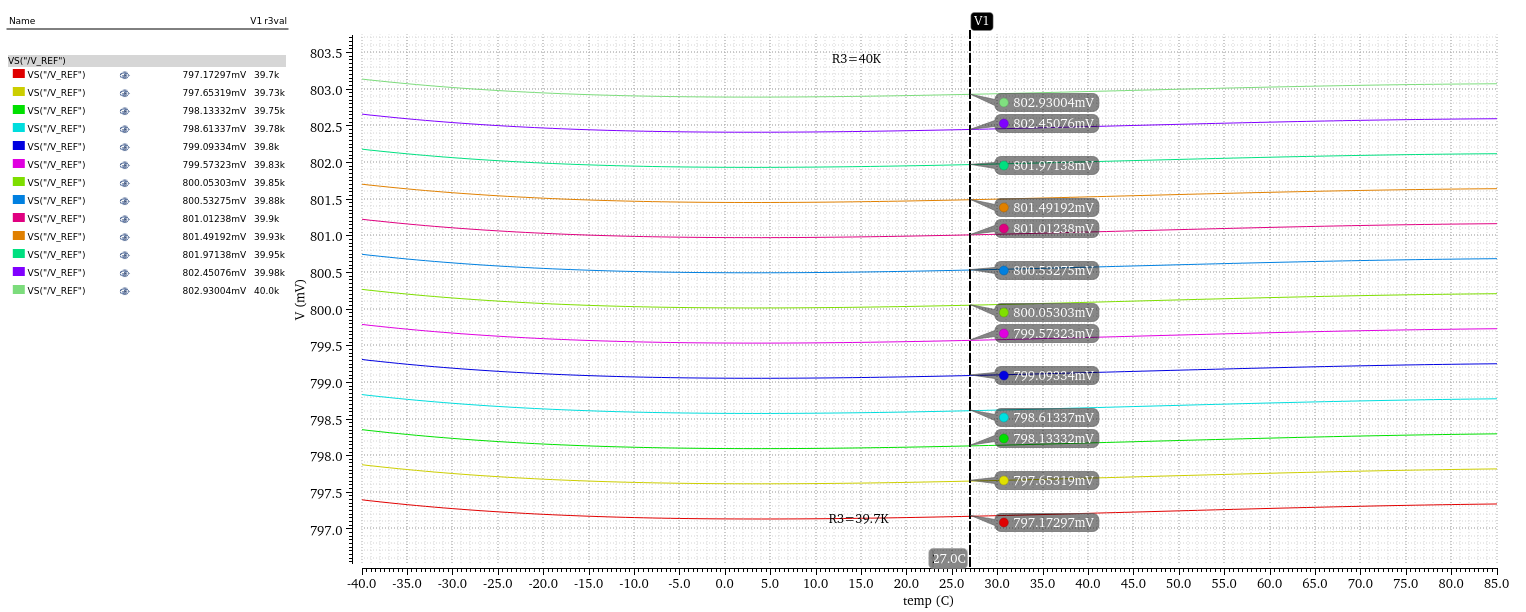
\includegraphics[width=\linewidth]{chapters/lab04/tuning3a.png}
    \caption{Parametric sweep of $R_3$ for setting $V_{REF}=0.8\,\mathrm{V}$.}
    \label{fig:tuning3a}
\end{figure}

The selected value is:
\[
\boxed{R_3=39.85\,\mathrm{k}\Omega}.
\]
The final temperature sweep is shown in Figure~\ref{fig:tuning3b}.

\begin{figure}[H]
    \centering
    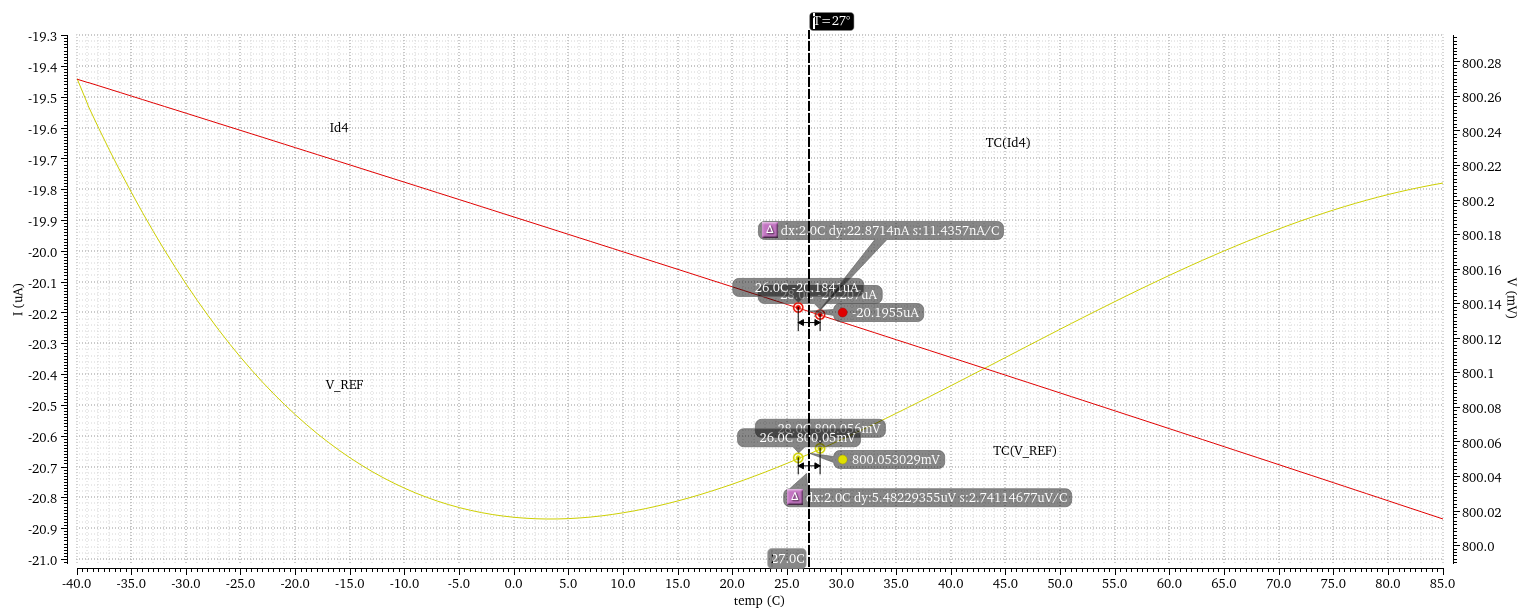
\includegraphics[width=\linewidth]{chapters/lab04/tuning3b.png}
    \caption{Final $V_{REF}$ and $I_{D4}$ after tuning $R_3$.}
    \label{fig:tuning3b}
\end{figure}

At room temperature:
\[
V_{REF}(27^\circ\mathrm{C})\approx800.05\,\mathrm{mV},
\qquad
\frac{dV_{REF}}{dT}\approx2.74\,\mu\mathrm{V/^\circ C},
\]
thus
\[
TC_{VREF} = \frac{1}{V_{REF}}\frac{dV_{REF}}{dT} \approx3.4\,\mathrm{ppm/^\circ C}.
\]
The $V_{REF}(T)$ characteristic exhibits a slight second-order curvature due to effects neglected in the hand calculations, mainly the temperature dependence of parameters such as $I_{S0}$. Nevertheless, the tuning keeps the room-temperature operating point on the flat part of the parabola, where the local temperature coefficient is small.

Since the local slope depends on where it is evaluated, the reference is also characterised over the whole temperature range with the box method:
\[
TC_{VREF}^{box} = \frac{V_{REF,max}-V_{REF,min}}{V_{REF}(27^\circ\mathrm{C})\,(T_{max}-T_{min})}
\approx \frac{800.27\,\mathrm{mV}-800.02\,\mathrm{mV}}{800.05\,\mathrm{mV}\cdot125^\circ\mathrm{C}}
\approx 2.5\,\mathrm{ppm/^\circ C},
\]
where $V_{REF,max}$ occurs at $-40^\circ\mathrm{C}$ and $V_{REF,min}$ at about $0^\circ\mathrm{C}$. Over the full $-40$ to $85^\circ\mathrm{C}$ range, the total variation is only about $0.25\,\mathrm{mV}$. The vertex of the parabola sits near $0^\circ\mathrm{C}$ rather than at the centre of the range ($22.5^\circ\mathrm{C}$). A slightly smaller $R_2$, which reduces the PTAT contribution, would move the vertex towards the centre and balance the two ends, lowering the box-method coefficient further.

Similarly,
\[
I_{D4}(27^\circ\mathrm{C})\approx20.20\,\mu\mathrm{A},
\qquad
\frac{dI_{D4}}{dT}\approx11.4\,\mathrm{nA/^\circ C}.
\]
Unlike $V_{REF}$, the internal branch currents are not directly optimized for temperature compensation. Therefore, a residual temperature dependence of $I_{D4}$ is expected after the tuning procedure.


\section{$V_{DD}$ Sensitivity}

Finally, the dependence of the reference voltage on the supply voltage was evaluated by performing a $V_{DD}$ sweep around its nominal value $1.2\,\mathrm{V}$. As required by the laboratory specifications, the supply voltage was varied within a $\pm10\%$ range:
\[
1.08\,\mathrm{V} \leq V_{DD} \leq 1.32\,\mathrm{V}.
\]

\begin{figure}[H]
    \centering
    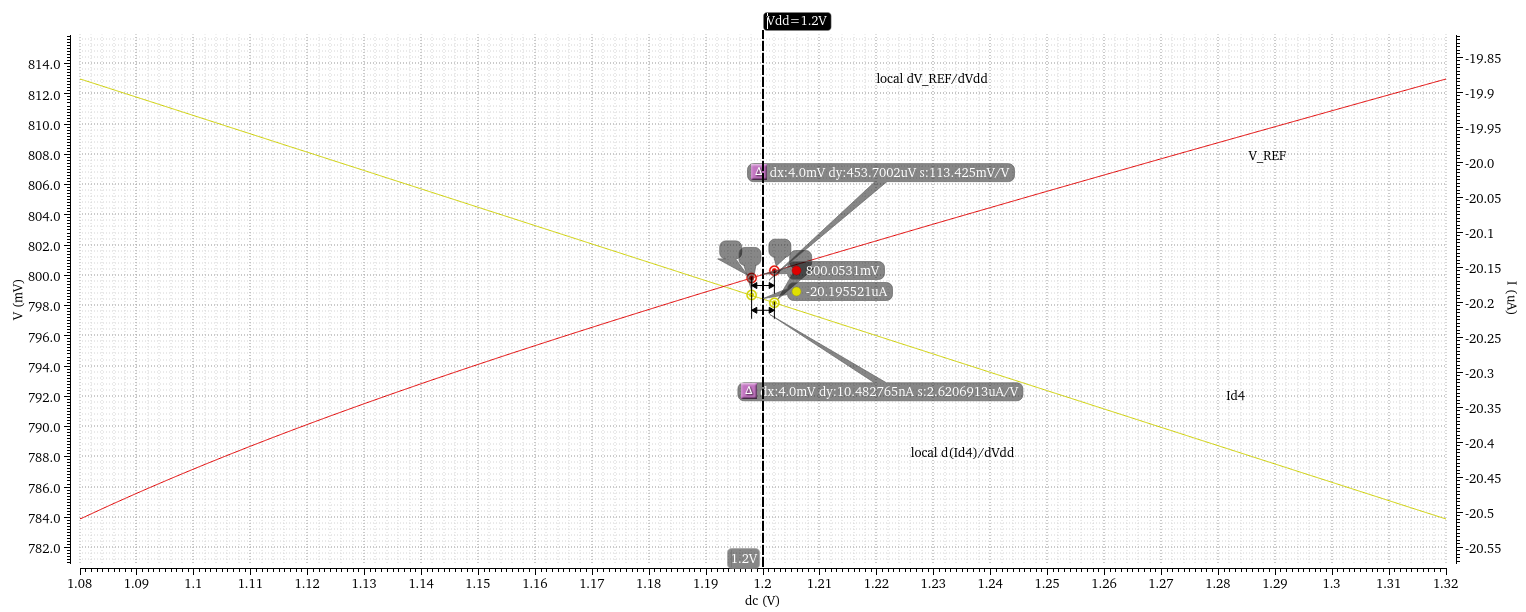
\includegraphics[width=\linewidth]{chapters/lab04/FINALFIG.png}
    \caption{$V_{REF}$ and $I_{D4}$ sensitivity to $V_{DD}$.}
    \label{fig:vdd_sensitivity}
\end{figure}

At $V_{DD}=1.2\,\mathrm{V}$, the reference voltage is approximately $V_{REF}\approx800.05\,\mathrm{mV}$. Using local markers around the nominal supply voltage, the sensitivity was estimated as:
\[
\frac{dV_{REF}}{dV_{DD}} \approx \frac{V_{REF}(1.202\,\mathrm{V})-V_{REF}(1.198\,\mathrm{V})}{4\,\mathrm{mV}} \approx113\,\mathrm{mV/V}.
\]

Similarly, the PMOS mirror current sensitivity is:
\[
\frac{dI_{D4}}{dV_{DD}} \approx \frac{I_{D4}(1.202\,\mathrm{V})-I_{D4}(1.198\,\mathrm{V})}{4\,\mathrm{mV}} \approx2.62\,\mu\mathrm{A}/\mathrm{V}.
\]
The final design therefore shows a good robustness against temperature variations, achieving a low local temperature coefficient around room temperature. On the other hand, the reference voltage is more sensitive to supply variations, as expected for a simple bandgap architecture without dedicated enhancement techniques.


\section{Final design verification}

The final design provides a reference voltage of $V_{REF}(27^\circ\mathrm{C})\approx800.05\,\mathrm{mV}$ with a local temperature coefficient of $TC_{VREF}\approx3.4\,\mathrm{ppm/^\circ C}$ at room temperature and a box-method coefficient of about $2.5\,\mathrm{ppm/^\circ C}$ over $-40$ to $85^\circ\mathrm{C}$ (total variation $\approx0.25\,\mathrm{mV}$). Although slightly higher than the target specification of $2\,\mathrm{ppm/^\circ C}$, this result confirms the effectiveness of the PTAT/CTAT compensation strategy and highlights the impact of second-order temperature effects neglected in the analytical derivation.

The dependence of the reference voltage on the supply voltage was also evaluated. Around the nominal supply voltage ($V_{DD}=1.2\,\mathrm{V}$), the measured sensitivity is:
\[
\frac{\mathrm{d}V_{REF}}{\mathrm{d}V_{DD}} \approx 113\,\mathrm{mV/V}
\]

